
Replay attacks are emulated according to the approach described in Section~\ref{ssec:replay}.
{\bfseries Needed here is an explanation of why you ignored $mic(t)$ and $a(t)$.}  Emulations include a random mix of three different loudspeakers impulse responses $spk(t)$ and three different replay environments $b(t)$.  Speaker impulse responses were obtained from~\cite{Brown2014} and correspond to a low-quality smartphone speaker, a medium-quality tablet speaker and a high-quality standalone speaker.  The impulse response and frequency responses of each are illustrated in Fig.~\ref{fig::IRs}.  There are significant differences in the frequency responses which show in particular the high-pass functions of the lower quality devices.

The first two replay environment impulse responses were obtained from~\cite{Jeub2009} and correspond to an enclosed medium-sized office and an open corridor.  The impulse and frequency responses of each are illustrated in Fig.~\ref{fig::Room_IRs}.  {\bfseries Not sure what these show??  No significant differences as far as I can see.  Consider removing them.}  The third impulse response simulates an anechoic chamber with a flat frequency response. 


\begin{figure}
	\centering
	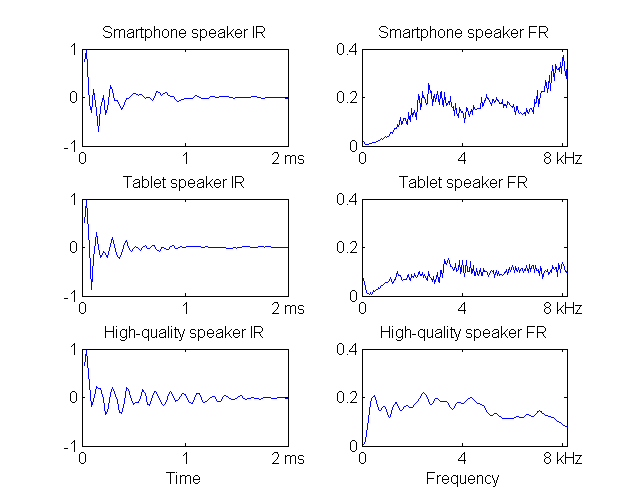
\includegraphics[width=1\linewidth]{Figs/IRs.png}
	\caption{Impulse left) and frequency (right) responses for three different speakers. {\bfseries Crop graphs so that they fit the linewidth fully.  Increase font size.  Label time axes in time, not samples.}}
	\label{fig::IRs}
\end{figure}


\begin{figure}
	\centering
	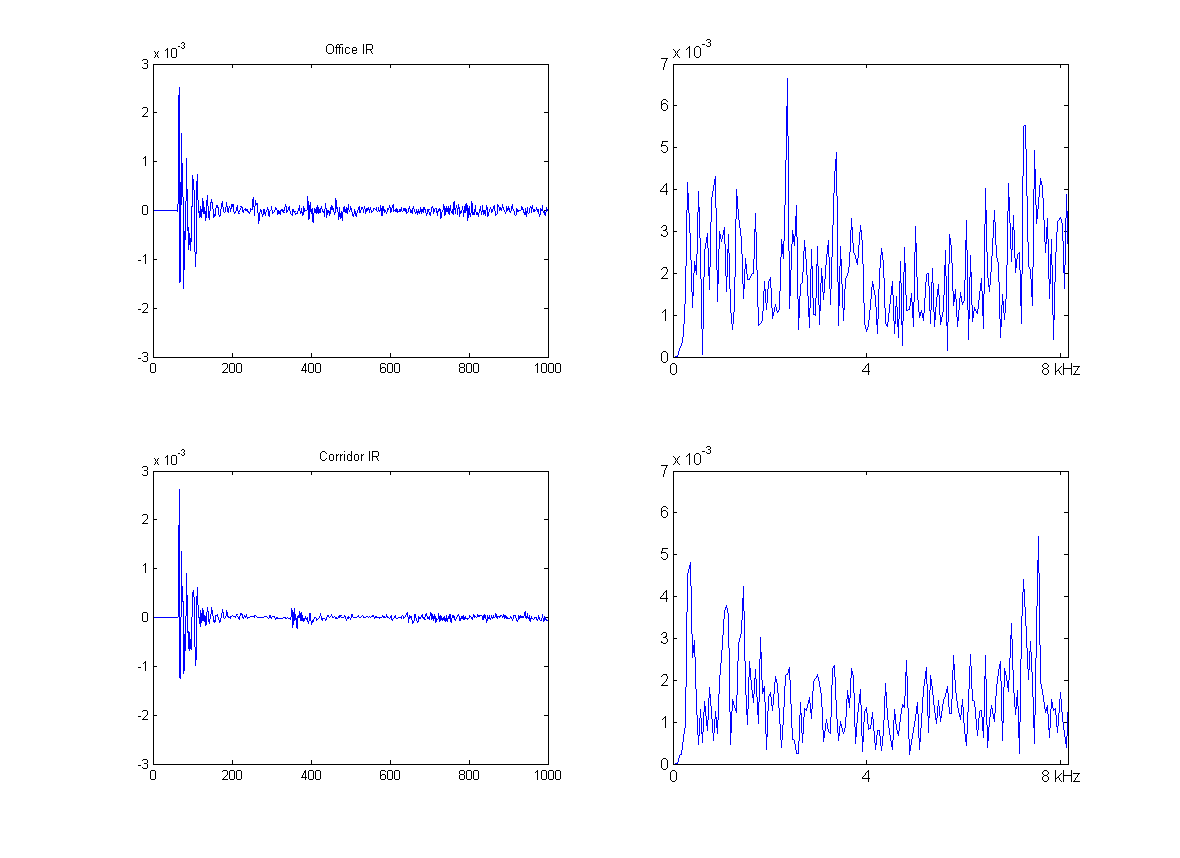
\includegraphics[width=1\linewidth]{Figs/Room_IRs.png}
	\caption{Impulse (left) and frequency (right) responses for two different replay environments.}
	\label{fig::Room_IRs}
\end{figure}


One potential problem here: in the use case relevant to this work, voice conversion speech synthesis and replay attacks will all involve replay, and thus a particular $b(t)$, yet your experiments only consider $b(t)$ for replay.  The comparison is therefore not fair.  I suggest to remove $b(t)$ in your replay work.  In any case there is no difference between the two impulse responses.